\section{Preliminaries, Definitions}\label{sec:prelims}

We begin by introducing the necessary definitions and terminology, as
well as a few observations about the mathematical objects of interest
which will be of use later.  We carefully lay out these definitions so
as to align with an intuitive understanding of the concepts and to
appease the astute reader who may be concerned with edge cases,
geometric weirdness, and nonmeasurability.  We use $\R^2$ to denote the 
Euclidean plane with its usual metric;
similarly, $\R^3$ denotes Euclidean 3-space.  We use $\mbb{S}^2$ to denote the \textit{unit 2-sphere}, which can be 
thought of as the set of points in $\R^3$ at Euclidean distance one from the origin.  In notation.

This surface also has a `usual metric', but it is tricky to write down as a formula.   Intuitively, the distance between two points on the sphere can be found by drawing the \textit{great circle} which passes through these points and then using a circular arc length formula to compute the length of the shorter of the two segments which join the points. 


We leave the consideration of
other surfaces, measures, and metrics to future work.

Before diving into the proofs, we present a quick gauntlet of definitions to establish the some working vocabulary.


\begin{definition}
  A \textbf{region} $\Omega$ in $\mathbb{S}^2$ or 
  in $\R^2$ is a non-empty open set together with its
  boundary, such that $\Omega$ is compact and the boundary can be described piecewise as 
  a finite collection of smooth curves.
\end{definition}

This definition is highly technical to allow us to assume away any annoying edge 
cases that might crop up.  Piece-by-piece, a \textit{non-empty open set} lets us 
talk about the \textit{area} of a region in a sensible way. Specifying that a region 
must be \textit{compact} gets rid of cases where we have to worry about regions having 
infinite area.  The entire plane should not be considered a `region'.  Finally, the 
\textit{piecewise-smooth boundary} condition gives us a way to talk about the \textit{perimeter} 
of a region.  We don't want to have to worry about fractal-like shapes which have well-defined 
area but an infinite perimeter.


\begin{definition}
	In a metric space, a \textbf{geodesic} between two points is the shortest path connecting them with respect to the metric.
	In the plane, geodesics are line segments, and on the surface of the sphere, geodesics are segments of great circles.
\end{definition}

\begin{definition}
  A \textbf{compactness score function} $\mathcal{C}$ is a function from
  the set of all regions to the positive real numbers.  We adopt the
  convention that a region with a \textit{higher} compactness score is
  \textit{more} compact, and this naturally induces a partial order over
  the set of all regions, where $A$ is at least as compact as $B$ if and
  only if $\mathcal{C}(A)\geq \mathcal{C}(B)$.
\end{definition}

The final major definition we need is that of a \textit{map
projection}.  In reality, the regions we are interested in comparing
sit on the surface of the Earth (i.e. a sphere), but these regions are
often examined after being projected onto a flat sheet of paper or
computer screen, and so have been subject to such a projection.

\begin{definition}
  A \textbf{map projection} $\varphi$ is a 
  diffeomorphism from a region on the sphere to a region on the 
  plane. 
\end{definition}

Intuitively, a map projection is a well-defined, invertible function between the sphere and the plane which sends regions on the sphere to regions in the plane.  Throughout, we use $\vphi$ to denote such a function from a region of the sphere 
to a region of the plane and $\vphi^{-1}$ its inverse, which goes from a region of the plane to a region of the sphere.

\begin{definition}
  We use the word \textbf{transformation} [of the plane/sphere] to mean
  to a diffeomorphism from the plane or sphere to itself.
\end{definition}

Since the image of a region under a map projection $\varphi$ is also
a region, we can examine the compactness score of that region both 
before and after applying $\varphi$, and this is the heart of the
problem we address in this paper.  We demonstrate, for several
examples of compactness scores $\mathcal{C}$, that the order
induced by $\mathcal{C}$ is different than the order induced by
$\mathcal{C}\circ\varphi$ for \textit{any} choice of map projection
$\varphi$.

\begin{definition}
  We say that a map projection $\vphi$ \textbf{preserves the  
  compactness score ordering} of a score $\mc{C}$ if for any regions 
  $\Omega,\Omega'$ in the sphere, $\mc{C}(\Omega)\ge \mc{C}(\Omega')$ 
  if and only if $\mc{C}(\vphi(\Omega)) \ge \mc{C}(\vphi(\Omega'))$ in the plane.
\end{definition}

   This is a weaker condition than simply preserving the raw compactness scores. 
   If there is some map projection which results in adding $.1$ to the score of each region, the raw scores are certainly not preserved, but the ordering of regions by their scores is. Additionally, $\vphi$ preserves a compactness score ordering 
  if and only if $\vphi^{-1}$ does.


\zs{this should be moved to the geometry section}
\begin{definition}
  A 
  \textbf{cap} on the sphere  $\mbb{S}^2$ is a region on the sphere
 which can be described as all of the points on the sphere to one side of some plane 
 in $\R^3$.  A cap has a \textit{height}, which is the largest distance between this cutting plane and the cap, and a \textit{radius}, which is the radius of the circle formed by the intersection of the plane and the sphere.  See \Cref{fig:caphr} for an illustration.
\end{definition}


\begin{figure}[h]
  \centering
  %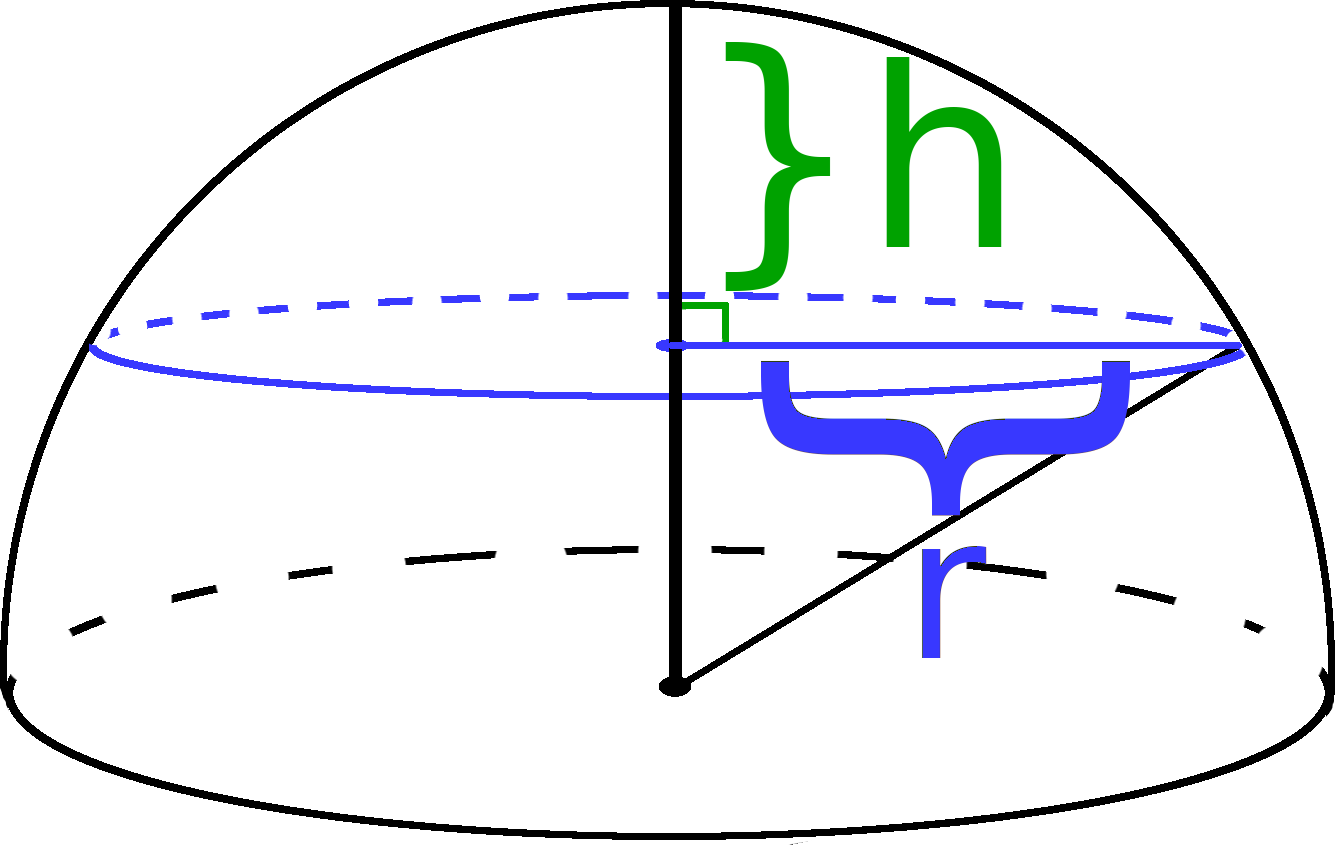
\includegraphics[width=.3\textwidth]{figs/spherecapschema}\\[1.5em]
  \definecolor{qqqqff}{rgb}{0,0,1}

\definecolor{ccqqqq}{rgb}{0.8,0,0}

\definecolor{ududff}{rgb}{0.30196078431372547,0.30196078431372547,1}

\begin{tikzpicture}[line cap=round,line join=round,>=triangle 45,x=1cm,y=1cm]

\clip(-4.493355050909743,-1.2748355780287404) rectangle (4.462150807191927,4.785872976331056);

\draw [shift={(0,0)},line width=3.2pt]  plot[domain=0:3.141592653589793,variable=\t]({1*4*cos(\t r)+0*4*sin(\t r)},{0*4*cos(\t r)+1*4*sin(\t r)});

\draw [shift={(0.0016366799970421299,9.441278259356354)},line width=2pt]  plot[domain=4.286394541961201:5.138764290071874,variable=\t]({1*7.708897306730456*cos(\t r)+0*7.708897306730456*sin(\t r)},{0*7.708897306730456*cos(\t r)+1*7.708897306730456*sin(\t r)});

\draw [shift={(0.019848790872865698,-6.481795867514522)},line width=2pt,dotted]  plot[domain=1.22830273729039:1.9174384984929125,variable=\t]({1*9.441973016351305*cos(\t r)+0*9.441973016351305*sin(\t r)},{0*9.441973016351305*cos(\t r)+1*9.441973016351305*sin(\t r)});

\draw [line width=2pt,color=ccqqqq] (0,2.4033620491027756)-- (0,4);

\draw [line width=2pt,color=qqqqff] (0,2.4033620491027756)-- (3.2001911763834157,2.3997450770024993);

\begin{scriptsize}

\draw [fill=ududff] (0.0016366799970421299,9.441278259356354) circle (2.5pt);

\draw [fill=ududff] (0.019848790872865698,-6.481795867514522) circle (2.5pt);

\draw[color=ccqqqq] (0.26805571312169243,3.3034918797019284) node {\LARGE$h$};

\draw[color=qqqqff] (1.6285727817769453,2.167711482419824) node {\LARGE $r$};

\end{scriptsize}

\end{tikzpicture}
  \caption{ The height $h$ and radius $r$ of a spherical cap. }
  \label{fig:caphr}
\end{figure}





